\documentclass{article}
\pagenumbering{gobble}
\title{Analysis of Fekete Points}
\author{Jesse Chan, Joseph Munar}
\date{}

\usepackage{amsmath}
\usepackage{graphicx}
\usepackage{csvsimple,booktabs,array,siunitx}
\usepackage{filecontents}

\begin{document}
\maketitle
\nopagebreak
\begin{abstract}
This article attempts to analyze the effectiveness of Spline interpolation and applications using Fekete points. First, we attempt to recreate 1-Dimensional Gauss-Legendre-Lobatto points from Fekete points. We then proced to demonstrate a formulation of variable problems for PDEs as well as an optimization to this process. Then we perform an error analysis on interpolation points using Fekete points for various maximum polynomial degrees and different sized knot vectors. We then compare the results to those performed for Gauss-Legendre-Lobatto points, uniform points, and Greville Abscissae. The report concludes with results and notes on the collocation procedure and optimization.
\end{abstract}
\section*{Introduction}
\paragraph{}
Fekete Points are known to be the Gauss-Legendre-Lobatto points for the line and its tensor products, and has been determined to be an adequate approximation of Gauss-Legendre-Lobatto points on the traingle and its tensor products. (cite here) has determined an approach to calculating Fekete points which allows further study into its applications. In this article, we analyze the effectiveness of Fekete points for interpolation using B-splines. A general algorithm for calculating B-splines was created by deBoor. He also showed a very important note for this article: that the condition number of a B-spline basis increases exponentially as K increases.

\section*{Fekete Points}
\paragraph{}
We begin with the realization that GLL points are calculated using the standard Lagrange basis, and thus utilizes the standard Vandermonde matrix. The easiest way to extrapolate this to a higher tensor product of lines in singular dimension is by projecting this interpolation over fixed intervals within the domain. As such, utilizing Spline spaces is the most appropriate direction for this project.

\subsection*{Spline Basis}
A general Spline Basis (or B-Spline) for this project will be defined as: A basis of piecewise polynomials of max N degrees. Spline spaces are constructed using a knot vector \textbf{t}
\begin{equation*}
\textbf{t}=\left\{a=t_1,...,t_{N+K+1}=b\right\},\qquad t_i<t_{i+1}.
\end{equation*}
where K is the number of non-overlapping sub-intervals within the spline space. The B-splines can thus be calculated recursively using:
\begin{equation*}
B^0_i(x)=\begin{cases}
1,\quad t_i\leq x\leq t_{i+1}\\
0,\quad otherwise.
\end{cases}
\qquad
B^K_i(x)=\frac{x-t_i}{t_{i+N}-t_i}B^{K-1}_i(x)+\frac{t_{i+N+1}-x}{t_{i+N+1}-t_{i+1}}B^{K-1}_{i+1}(x).
\end{equation*}

\subsection*{Interpolation}
\paragraph{}
To achieve a unique solution to a spline interpolation, the knot vector must contain $N+1$ copies of the boundary terms, and there must be $N+K$ interpolation points. This allows for the existence of a square matrix which contains the coefficients of the B-splines for a unique set of interpolation points and knot vector. The entries of this matrix can be calculated using deBoor$'$s algorithm. This matrix will be referred to in this article as the Spline Vandermonde matrix. Inverting the Spline Vandermonde matrix gives the solution vector to the interpolation points.

\subsection*{Fekete Points Generation Algorithm}
\paragraph{}
A gradient ascension algorithm was used to generate the Fekete points for this project. As explained by (insert cite), one can apply $\frac{d\phi_i}{dr_i}$ to the $i\textsuperscript{th}$ node in the set of interpolation points recursively. Fekete points are achieved once 
\begin{equation*}\frac{d\phi_i}{dr_i}\leq 10^{-12}.\end{equation*}

Since we are working with a square Spline Vandermonde matrix, then $\frac{d\phi_i}{dr_i}$ for all global nodes will be the diagonal entries of the square derivative matrix. In general, the derivative of a spline can be calculated through the same method as the spline itself, but will be of max $N-1$ degrees and have a knot vector similar to the original spline but with the interior points duplicated. However, these derivatives are only locally defined, and require a map that will lead us to the global derivatives we desire. Applying a time stepping scheme such as Forward Euler or Runge Kutta 45 to the set of interpolation points and diagonal entries of the now-square derivative matrix give the desired Fekete interpolation points. As a precautionary check, setting $K=1$ in the algorithm should provide Fekete points that are equivalent to GLL points for any N.
\newline\newline\newline\hspace*{-0.5cm}
\includegraphics[height = 5cm]{K_1_check.png} \includegraphics[height = 5cm]{K_1_error.png}

\section*{Variational Formulation for Time Dependent Problems}
\subsection*{Finite Element Formulation}
\paragraph{}
Next, we attempt a classic finite element method approach to time dependent partial differential equations using B-Splines. We$'$ll attempt this on the 1-D Wave Equation with homogeneous Neumann boundary and initial conditions: 
\begin{equation*}
\frac{\partial ^2 u}{\partial t^2} = c^2\frac{\partial ^2 u}{\partial x^2},\quad \frac{\partial u}{\partial x}(-1,t)=\frac{\partial u}{\partial x}(1,t)=0, \frac{\partial u}{\partial t}(x,0)=0
\end{equation*}
Where $c$ is a constant and $u$ is a solution function dependent on variables $x$ and $t$. Inserting a test function, $v(x)$, and integrating gives: 
\begin{equation*}
\int \frac{\partial ^2 u(x,t)}{\partial t^2}v(x)dx = c^2\int \frac{\partial ^2 u(x,t)}{\partial x^2}v(x)dx
\end{equation*}
Applying a discretization, $u(x,t) = \sum a(t)\phi(x)$, and invoking the boundary conditions simplifies the equation into a linear system:
\begin{equation*}
\frac{\partial ^2\vec{a}}{\partial t^2}M + c^2\vec{a}K=0
\end{equation*}
where M is the mass matrix and K is the stiffness matrix defined as:
\begin{equation*}
M_{i,j}=\int ^1_{-1}\phi _i(x)\phi _j(x)dx,\qquad K_{i,j}=\int ^1_{-1}\frac{\partial \phi _i}{\partial x}\frac{\partial \phi _j}{\partial x}dx
\end{equation*}
These equations can be solved using quadrature approximations:
\begin{equation*}
M_{i,j}=\sum _{i,j=0}^N w_i\phi _i(x)\phi _j(x),\qquad K_{i,j}=\sum _{i,j=0}^N w_i\frac{\partial \phi _i}{\partial x}\frac{\partial \phi _j}{\partial x}
\end{equation*}
Where $w_i$ is the weight of the $i\textsuperscript{th}$ interpolation point. To easily calculate these weights, we used Gaussian Quadrature points. Using a Forward Euler approach, we get an explicit time leapfrogging method:
\begin{equation*}
\vec{a}^{(t+2)} = -M^{-1}K\vec{a}^{(t+1)}(c\times dt)^2+2\vec{a}^{(t+1)} - \vec{a}^{(t)}
\end{equation*}

\subsection*{Mass-Lumping}
\paragraph{}
As for any explicit time stepping scheme, the mass matrix must be solved. However, these matrices are completely dense, and inversion quickly becomes less feasible and more numerically taxing as $K$ and $N$ increase. We wish to simplify this hardship by replacing the dense matrix with a diagonal matrix - a mass-lumped matrix. For this, we switch from Gaussian Quadrature points to a set of nodal points such as GLL points. Since we already have calculated the weights of the Gaussian Quadrature points and we can easily calculate the quadrature matrices of both types of points, we can derive the weights of the GLL points using: 
\begin{equation*}
(qG)^T\times \vec{wG}=(qQ)^T\times \vec{wQ}
\end{equation*}
where $qG$ and $qQ$ are the quadrature matrices for GLL and Gaussian Quadrature points, and $\vec{wG}$ and $\vec{wQ}$ are their respective weight vectors. Choosing to use Fekete points allow us to utilize the increased accuracy provided from the subintervals of the B-Spline basis. Using a nodal basis forces the Spline Vandermonde matrix to be the identity matrix. Therefore, the now-mass-lumped mass matrix, $M_L$ is defined as:
\begin{equation*}
M_{L_{i,j}}=\begin{cases}
\vec{wG}_i,\quad i=j\\ 0,\quad otherwise.
\end{cases}
\end{equation*}

\section*{Numerical Experiments}
\subsection*{Convergence of Time-Stepping to Achieve Fekete Points}
\paragraph{}
Part of any gradient ascension algorithm is the time-step needed. In the case of this generation algorithm, it seems a very small time-step is needed. Through experimentation, it was observed that a higher N and/or K requires a smaller time-step. This is most likely a side effect of the Spline Vandermonde matrix becoming more unstable with higher N and K. A suitable formula to determine the time step needed seems to be $dt = \frac{1}{200\times N\times K}$

\subsection*{Analysis on Fekete Points and Greville Abscissae}
\paragraph{}
Greville Abscissae are the averages of a knot vector. Because of this, they have been used extensively for interpolation using B-Splines. Initial error analysis of the two types of interpolation points show they have very similar results.
\paragraph{}
Further inspection of the points show they are almost identical. As N and K increase, more interior points of both types of interpolation points converge to the same results. The exterior points will never be the same due to how they are defined. For all other points, Fekete points seem to be more spread out whereas Greville abscissae seem to clump more towards the middle of the knot vector.
\hspace*{-2cm}\includegraphics[width = 8cm]{Difference_N_2.png}\includegraphics[width = 8cm]{Difference_N_3.png}
\hspace*{-2cm}\includegraphics[width = 8cm]{Difference_N_4.png}\includegraphics[width = 8cm]{Difference_N_7.png}
\subsection*{Interpolation Errors}
\paragraph{}
We first examine the error for two smooth functions using GLL points, Fekete Points, uniform points, and Greville abscissae. As previously mentioned, the Spline Vandermonde matrix has a higher condition number as K and N increase. This effect is seen in both the uniform points graph and the Fekete Points graph. Fekete Points are affected by this more than Greville Abscissae most likely because Fekete Points are generated using a B-spline basis. The results are shown below:
\newline\hspace*{-0.5cm}
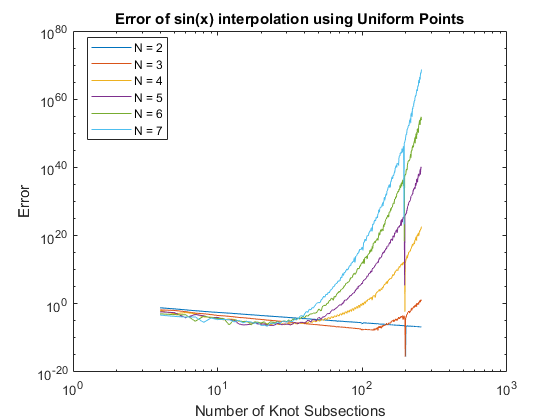
\includegraphics[height = 2.5cm]{SinUniform.png} 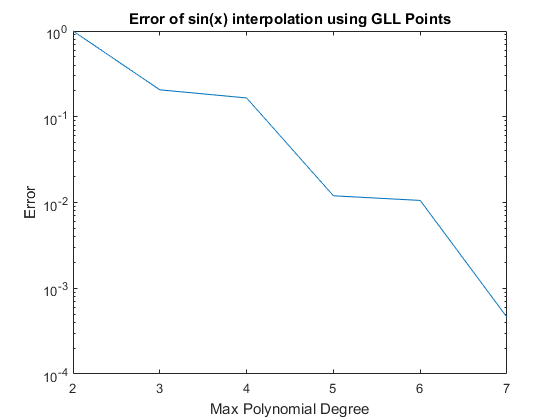
\includegraphics[height = 2.5cm]{SinGLL.png}
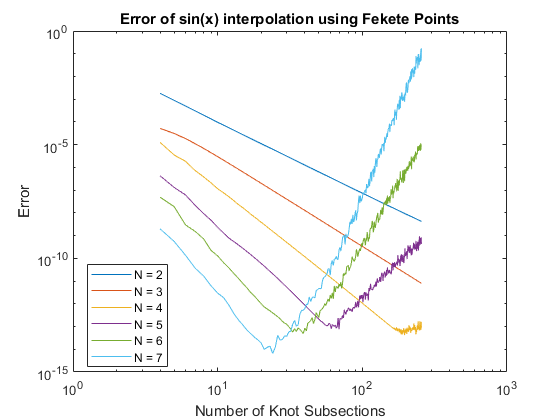
\includegraphics[height = 2.5cm]{SinFekete.png} 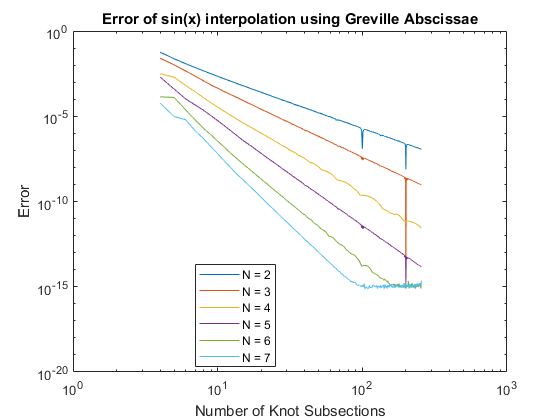
\includegraphics[height = 2.5cm]{SinGreville.png}
\hspace*{-0.5cm}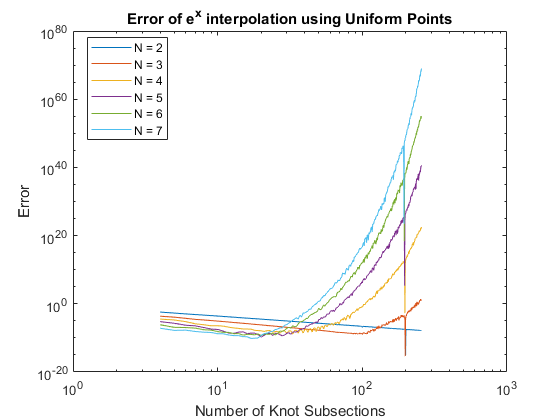
\includegraphics[height = 2.5cm]{ExpUniform.png} 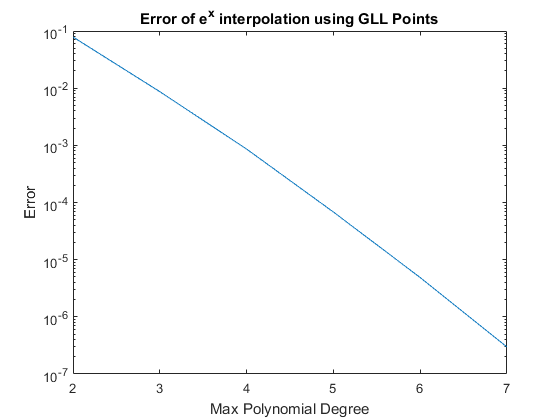
\includegraphics[height = 2.5cm]{ExpGLL.png}
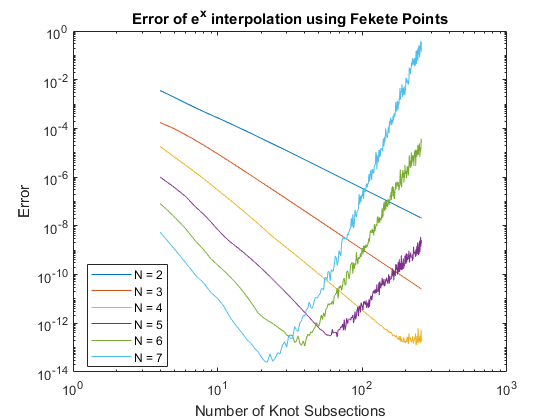
\includegraphics[height = 2.5cm]{ExpFekete.png} 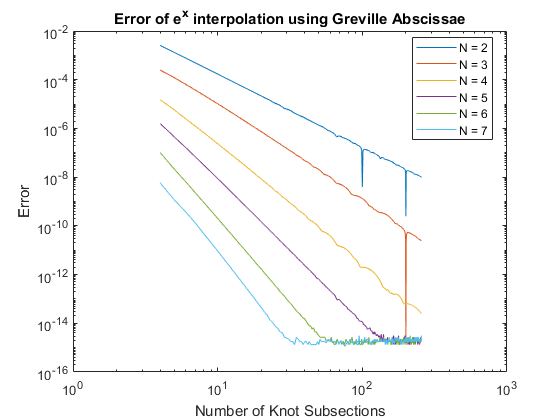
\includegraphics[height = 2.5cm]{ExpGreville.png}

\paragraph{}
We then decided to examine the error for two smooth functions that experience the Runge phenomenon when interpolated. The same types of interpolation points were used. It was at this point where we first noticed the similarities between the Greville Abscissae and Fekete Points. Another important note is that a B-spline basis helps dramatically reduce the effects of Runge's Phenomenon:
\newline\hspace*{-0.5cm}
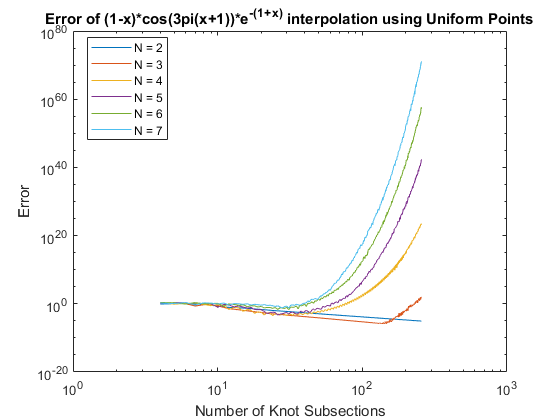
\includegraphics[height = 2.5cm]{CosExpUniform.png} 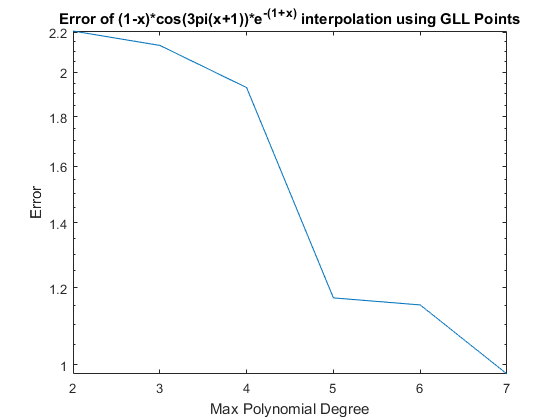
\includegraphics[height = 2.5cm]{CosExpGLL.png}
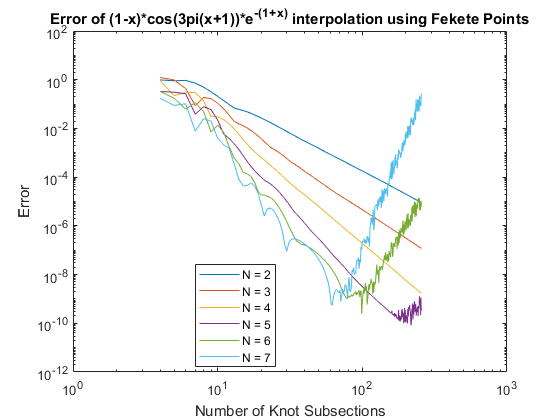
\includegraphics[height = 2.5cm]{CosExpFekete.png} 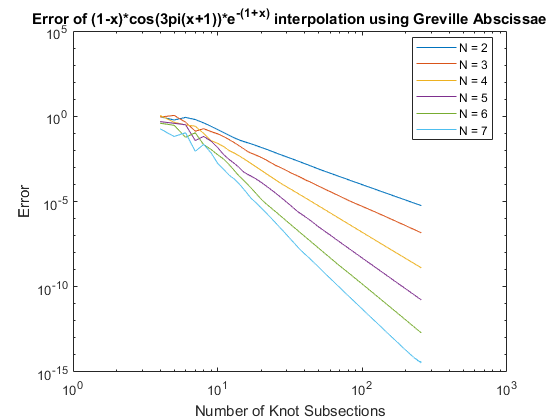
\includegraphics[height = 2.5cm]{CosExpGreville.png}
\hspace*{-0.5cm}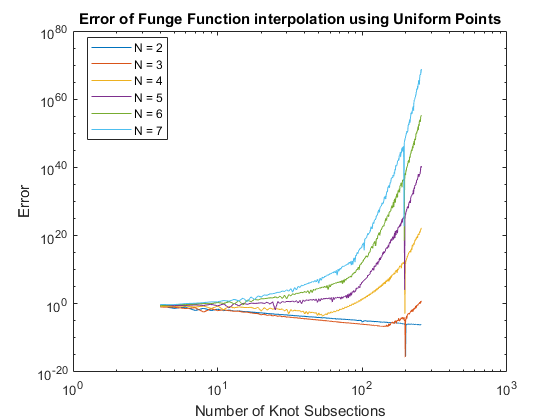
\includegraphics[height = 2.5cm]{RungeUniform.png} 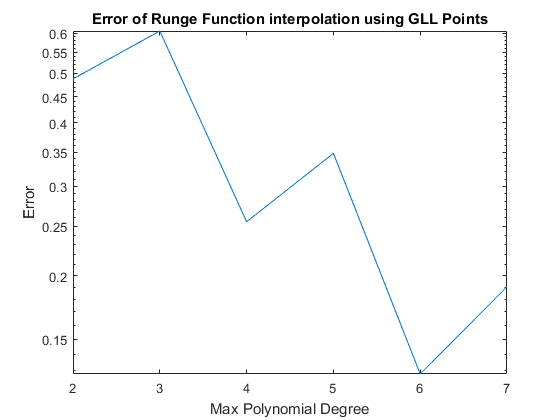
\includegraphics[height = 2.5cm]{RungeGLL.png}
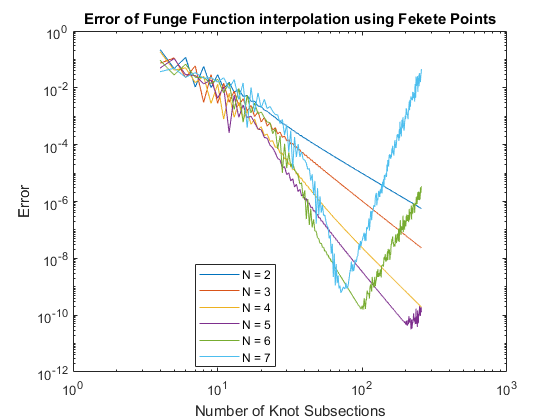
\includegraphics[height = 2.5cm]{RungeFekete.png} 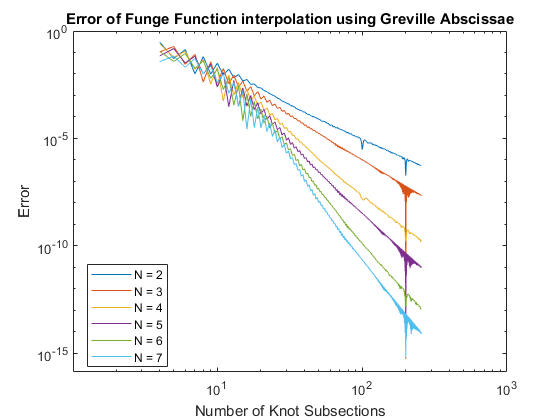
\includegraphics[height = 2.5cm]{RungeGreville.png}

\subsection*{Mass-Lumping}
The results of the mass lumping approximation for time, $t=1$ are below:
\newline\hspace*{-0.5cm}
\includegraphics[height = 5cm]{Wave_3rd_error.png} \includegraphics[height = 5cm]{Wave_4th_error.png}

An important note of this procedure: Fekete points are only an approximation of GLL points, this equation will also only be an approximation. Thus the derived weight vector may not be exact. The error, as a result, will increase at a higher rate than expected when using more than one sub-interval.


\section*{Appendix}
A list of Fekete points for $K=4-256$ for $N=2-7$ have been written into 6 Excel documents saved on the public Github repository.

\end{document}
